\documentclass[12pt, a4paper]{article}

\usepackage{amsmath, amssymb, amsthm}
\usepackage{geometry}
\usepackage{tikz}
\usetikzlibrary{angles, quotes, decorations.markings, calc}
\usepackage{microtype}

\geometry{margin=2.5cm}

% ── Larger, visible hat over the vertex letter only ─────────────────
% \overset{\wedge}{X} gives a clearly visible caret above X
\newcommand{\ang}[1]{\overset{\wedge}{#1}}

% ── Tick-mark styles for sides ──────────────────────────────────────
\tikzset{
  singletick/.style={
    postaction={decorate,
      decoration={markings,
        mark=at position 0.5 with {
          \draw[line width=0.7pt] (0pt,-3.5pt)--(0pt,3.5pt);
        }
      }
    }
  },
  doubletick/.style={
    postaction={decorate,
      decoration={markings,
        mark=at position 0.5 with {
          \draw[line width=0.7pt] (-2pt,-3.5pt)--(-2pt,3.5pt);
          \draw[line width=0.7pt] ( 2pt,-3.5pt)--( 2pt,3.5pt);
        }
      }
    }
  }
}

% ── Theorem-style environments ──────────────────────────────────────
\newtheoremstyle{criterion}
  {6pt}{6pt}{\normalfont}{0pt}{\bfseries}{.}{0.5em}{}
\theoremstyle{criterion}
\newtheorem*{SAS}{First Criterion of Congruence (SAS)}
\newtheorem*{ASA}{Second Criterion of Congruence (ASA)}

\title{\textbf{Congruence Criteria for Triangles}}
\author{0xHaru}
\date{\today}

\begin{document}

\maketitle
\thispagestyle{empty}

% ══════════════════════════════════════════════════════════════════════
\begin{SAS}
Two triangles are congruent if they have two sides and the included
angle between them respectively congruent.
\end{SAS}

\begin{center}
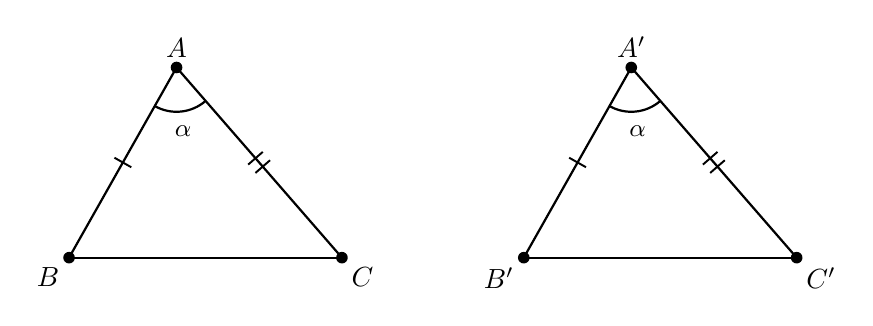
\begin{tikzpicture}[scale=1.05]
  % ── Triangle ABC ─────────────────────────────────────────────────
  \coordinate (A1) at (1.3, 2.3);
  \coordinate (B1) at (0,   0  );
  \coordinate (C1) at (3.3, 0  );

  \draw[thick, singletick] (A1) -- (B1);
  \draw[thick]             (B1) -- (C1);
  \draw[thick, doubletick] (A1) -- (C1);

  % angle at A with alpha label just outside the arc
  \draw pic["$\alpha$", draw=black, thick,
            angle radius=16pt,
            angle eccentricity=1.45,
            font=\small]
        {angle=B1--A1--C1};

  \foreach \p/\lbl/\anch in {A1/$A$/above, B1/$B$/below left, C1/$C$/below right}
    { \fill (\p) circle (2pt); \node[\anch] at (\p) {\lbl}; }

  % ── Triangle A'B'C' ───────────────────────────────────────────────
  \begin{scope}[xshift=5.5cm]
    \coordinate (A2) at (1.3, 2.3);
    \coordinate (B2) at (0,   0  );
    \coordinate (C2) at (3.3, 0  );

    \draw[thick, singletick] (A2) -- (B2);
    \draw[thick]             (B2) -- (C2);
    \draw[thick, doubletick] (A2) -- (C2);

    \draw pic["$\alpha$", draw=black, thick,
              angle radius=16pt,
              angle eccentricity=1.45,
              font=\small]
          {angle=B2--A2--C2};

    \foreach \p/\lbl/\anch in {A2/$A'$/above, B2/$B'$/below left, C2/$C'$/below right}
      { \fill (\p) circle (2pt); \node[\anch] at (\p) {\lbl}; }
  \end{scope}
\end{tikzpicture}
\end{center}

\bigskip

% ══════════════════════════════════════════════════════════════════════
\begin{ASA}
Two triangles are congruent if they have one side and the two angles
adjacent to it respectively congruent.
\end{ASA}

\begin{center}
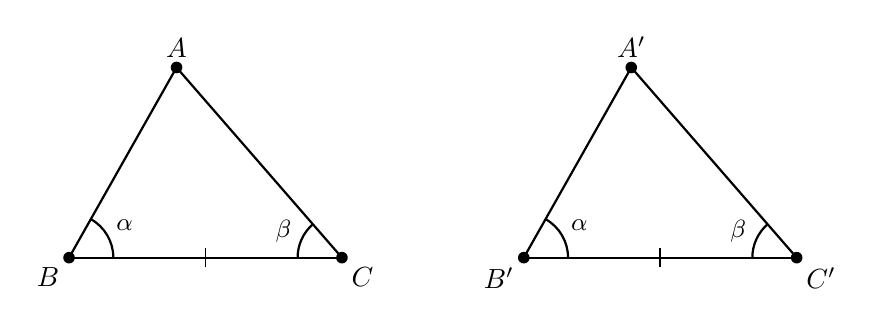
\begin{tikzpicture}[scale=1.05]
  % ── Triangle ABC ─────────────────────────────────────────────────
  \coordinate (A1) at (1.3, 2.3);
  \coordinate (B1) at (0,   0  );
  \coordinate (C1) at (3.3, 0  );

  \draw[thick]             (A1) -- (B1);
  \draw[thick, singletick] (B1) -- (C1);
  \draw[thick]             (A1) -- (C1);

  % angle at B — labelled alpha
  \draw pic["$\alpha$", draw=black, thick,
            angle radius=16pt,
            angle eccentricity=1.45,
            font=\small]
        {angle=C1--B1--A1};

  % angle at C — labelled beta
  \draw pic["$\beta$", draw=black, thick,
            angle radius=16pt,
            angle eccentricity=1.45,
            font=\small]
        {angle=A1--C1--B1};

  \foreach \p/\lbl/\anch in {A1/$A$/above, B1/$B$/below left, C1/$C$/below right}
    { \fill (\p) circle (2pt); \node[\anch] at (\p) {\lbl}; }

  % ── Triangle A'B'C' ───────────────────────────────────────────────
  \begin{scope}[xshift=5.5cm]
    \coordinate (A2) at (1.3, 2.3);
    \coordinate (B2) at (0,   0  );
    \coordinate (C2) at (3.3, 0  );

    \draw[thick]             (A2) -- (B2);
    \draw[thick, singletick] (B2) -- (C2);
    \draw[thick]             (A2) -- (C2);

    \draw pic["$\alpha$", draw=black, thick,
              angle radius=16pt,
              angle eccentricity=1.45,
              font=\small]
          {angle=C2--B2--A2};

    \draw pic["$\beta$", draw=black, thick,
              angle radius=16pt,
              angle eccentricity=1.45,
              font=\small]
          {angle=A2--C2--B2};

    \foreach \p/\lbl/\anch in {A2/$A'$/above, B2/$B'$/below left, C2/$C'$/below right}
      { \fill (\p) circle (2pt); \node[\anch] at (\p) {\lbl}; }
  \end{scope}
\end{tikzpicture}
\end{center}

% ══════════════════════════════════════════════════════════════════════
\subsection*{Proof of the Second Criterion}

\noindent
Let $ABC$ and $A'B'C'$ be two triangles such that
\[
  AC \cong A'C', \qquad A\ang{C}B \cong A'\ang{C'}B', \qquad
  C\ang{A}B \cong C'\ang{A'}B'.
\]
We want to show that $\triangle ABC \cong \triangle A'B'C'$.

\begin{center}
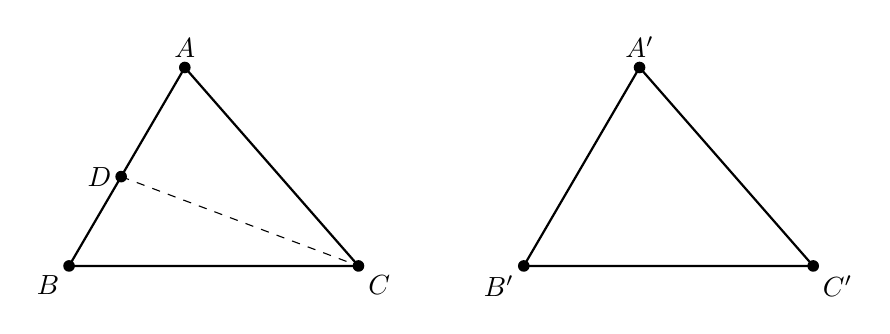
\begin{tikzpicture}[scale=1.05]
  % ── Triangle ABC with auxiliary point D on AB ────────────────────
  \coordinate (A1) at (1.4, 2.4);
  \coordinate (B1) at (0,   0  );
  \coordinate (C1) at (3.5, 0  );
  \coordinate (D1) at ($(A1)!0.55!(B1)$);

  \draw[thick] (A1) -- (B1) -- (C1) -- cycle;
  \draw[dashed] (D1) -- (C1);

  \fill (A1) circle (2pt) node[above]       {$A$};
  \fill (B1) circle (2pt) node[below left]  {$B$};
  \fill (C1) circle (2pt) node[below right] {$C$};
  \fill (D1) circle (2pt) node[left]        {$D$};

  % ── Triangle A'B'C' ───────────────────────────────────────────────
  \begin{scope}[xshift=5.5cm]
    \coordinate (A2) at (1.4, 2.4);
    \coordinate (B2) at (0,   0  );
    \coordinate (C2) at (3.5, 0  );

    \draw[thick] (A2) -- (B2) -- (C2) -- cycle;

    \fill (A2) circle (2pt) node[above]       {$A'$};
    \fill (B2) circle (2pt) node[below left]  {$B'$};
    \fill (C2) circle (2pt) node[below right] {$C'$};
  \end{scope}
\end{tikzpicture}
\end{center}

\noindent
Suppose, for contradiction, that the two triangles are \emph{not}
congruent. Since $AC \cong A'C'$ by hypothesis, the non-congruence must
involve at least one of the remaining sides; assume without loss of
generality that $AB > A'B'$. In this case we can take a point $D$ on
segment $AB$ such that $AD \cong A'B'$.

\medskip\noindent
Consider now triangles $ADC$ and $A'B'C'$. They satisfy:
\begin{enumerate}
  \item $AD \cong A'B'$, by construction;
  \item $AC \cong A'C'$, by hypothesis;
  \item $C\ang{A}D \cong C'\ang{A'}B'$, by hypothesis (since $D$ lies on
        ray $AB$, the angle $C\ang{A}D$ coincides with $C\ang{A}B$).
\end{enumerate}
By the \textbf{First Criterion of Congruence} (SAS), it follows that
$\triangle ADC \cong \triangle A'B'C'$.

\medskip\noindent
In particular, this congruence gives $A\ang{C}D \cong A'\ang{C'}B'$.
But by hypothesis $A'\ang{C'}B' \cong A\ang{C}B$, so
\[
    A\ang{C}D \cong A\ang{C}B.
\]
This is a contradiction: since $D$ lies \emph{strictly} between $A$ and
$B$, the ray $CD$ falls strictly inside the angle $A\ang{C}B$, which
forces $A\ang{C}D < A\ang{C}B$.

\medskip\noindent
The hypothesis of non-congruence is therefore absurd, and we conclude that
the two triangles are congruent.\hfill$\square$

\end{document}
